%/*******************************************************************************
% * Copyright (c) 2007, G. Weirich
% * All rights reserved. This program may not be distributed
% * or modified without prior written consent
% *
% * Contributors:
% *    G. Weirich - initial implementation
% *
% *  $Id: anleitung.tex 231 2007-08-23 19:12:43Z Gerry $
% *******************************************************************************/

\documentclass[a4paper]{scrartcl}
\usepackage{german}
\usepackage[utf8]{inputenc}
\usepackage{makeidx}
\usepackage[pdftex]{graphicx}
\DeclareGraphicsExtensions{.pdf,.jpg,.png}
\makeindex
\usepackage{floatflt}
\usepackage{wrapfig}
\usepackage[]{hyperref}
\usepackage{color}
\title{Elexis-Medikamente-BAG}
\author{Gerry Weirich}

\begin{document}
\maketitle
\section{Einführung}

Dies ist ein Medikamente-Plugin, das als Datenbasis die vom BAG veröffentlichte Excel\texttrademark-Version der Spezialitätenliste verwendet. Darüberhinaus hat es einige funktionelle Erweiterungen gegenüber dem älteren, Galdat-basierten Plugin. Es bindet sich in die Verrechnen-View und in die Artikel-Perspektive ein und kann so exakt gleich wie die anderen Verrechnungsbezogenen Views verwendet werden.

\section{Voraussetzungen}
Dieses Plugin benötigt Elexis 1.1.1 oder höher.

\medskip

Dieses Plugin kann entweder allein oder auch zusammen mit dem existierenden Galdat-Plugin verwendet werden. In letzterem Fall wird auch eine gemeinsame Datenbasis verwendet. Das heisst, bei Medikamenten der SL werden die zusätzlichen SL-spezifischen Angaben integriert, die nicht-SL-Artikel bleiben weiterhin vorhanden, aber haben weiterhin nur die Galdat-Informationen. (Die Zusätzlichen Informationen der SL-Medikamente sind im Wesentlichen Inhaltsstoffe, therapeutische Gruppe und Generika-Status)

\section{Verwendung}
\begin{figure}[htbp]
     \begin{minipage}{0.5\textwidth}
      \centering
       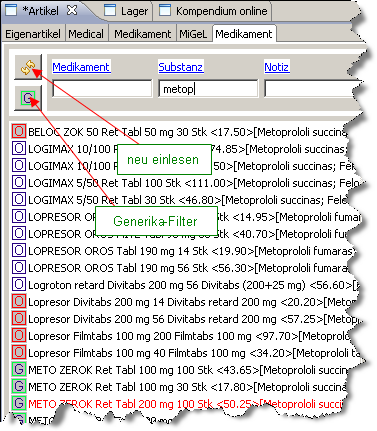
\includegraphics[width=0.9\textwidth]{liste1}
       \caption{Medikamente BAG}
       	\label{fig:bagmedi}
     \end{minipage}\hfill
     \begin{minipage}{0.5\textwidth}
      \centering
       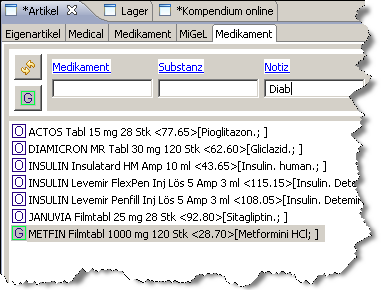
\includegraphics[width=0.9\textwidth]{liste2}
       \caption{Gruppierung nach Notiz}
       \label{fig:bagmedi2}
     \end{minipage}
\end{figure}

In der Listenauswahl (Abb. \ref{fig:bagmedi}) haben Sie jetzt einen Generika-Filterknopf und drei verschiedene Felder zur Auswahl:
\begin{itemize}
    \item Name: Medikamente nach Name filtern
    \item Substanz: Medikamente nach Inhaltsstoff filtern
    \item Notiz: Medikamente nach eigenen Notizen filtern.
\end{itemize}
Wenn der Generika-Knopf eingerastet ist, werden bei allen \textit{nachfolgenden} Filterungen nur Generika angezeigt.

\medskip

Wenn Sie auf ein Medikament mit der rechten Maustaste klicken, erhalten Sie ausserdem die Option "'selbe therap. Gruppe"'. Auswahl dieser Option bewirkt, dass alle Medikamente, die zur selben therapeutischen Gruppe gehören, angezeigt werden.

Die Bilder vor dem Medikamentennamen stehen für den Generikastatus: Blaues O bedeutet: Dies ist ein Originalpräparat, für das kein Generikum existiert. Rotes O bedeutet: Dies ist ein Originalpräparat, für das midnestens ein Generikum existiert. Grünes G bedeutet: Dies ist ein Generikum.

 Jede Zeile enthält den offiziellen Namen des Medikaments, dahinter den $<$Preis$>$, dann die [Inhaltsstoffe] und zuletzt, bei Lagerartikeln, den (Lagerbestand). Lagerartikel werden ausserdem in blau dargestellt, oder in rot, falls der Lagerbestand unter den Minimalbestand abgesunken ist.

\medskip

Die \textsc{Notiz}-Spalte (Abb. \ref{fig:bagmedi2}) dient dazu, Medikamente nach eigenen Kriterien zu gruppieren. Beispielsweise könnten Sie \glqq{}Ihren\grqq{} Diabetesmedikamenten die Notiz \textit{Diabetes} zuordnen. Wenn Sei dann im Notiz-Feld \textit{Diabetes} eintippen, erscheint Ihre Auswahl.

\medskip

Klick auf den \textsc{neu einlesen} Knopf löscht alle Filterbedingungen und lädt somit wieder alle Medikamente in die Liste.

\section{Detailansicht}
\begin{figure}
    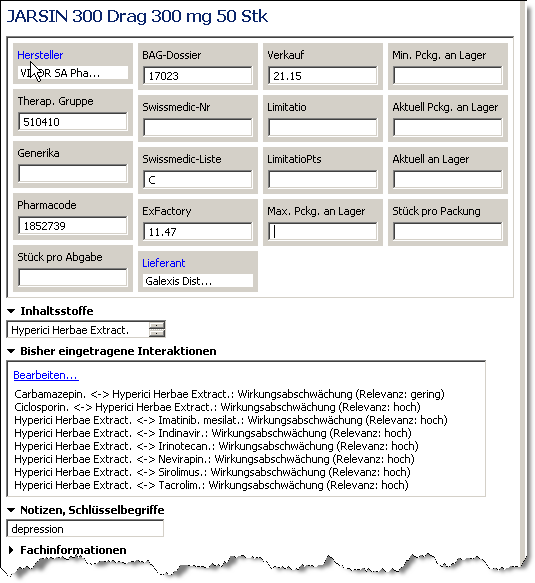
\includegraphics{detail1}
    \caption{Medikament-Detailansicht}
    \label {fig:bagdetail}
\end{figure}
Die Detailansicht zeigt Ihnen einerseits verschiedene Details zum ausgewählten Medikament, erlaubt Ihnen aber andererseits auch, eigene Ergänzungen anzubringen.

\subsection{Datenfelder}
Die Datenfelder im oberen Bereich bieten Ihnen die Möglichkeit, ein Medikament als Lagerartikel zu deklarieren. Gehen Sie dazu so vor:
\begin{itemize}
\item Geben Sie unter \textsc{Min. Pckg. an Lager} ein, wieviele Packungen dieses Medikaments mindestens an Lager sein sollen. (Sobald die vorhandene Anzahl unter diese Zahl fällt, wird das betreffende Medikament bei der nächsten Bestellung aufgeführt)
\item Geben Sie unter \textsc{Max. Pckg. an Lager} ein, wieviele Packungen dieses Medikaments höchstens an Lager sein sollen. Wenn eine Bestellung erstellt wird, dann werden soviele Packungen bestellt, dass diese Zahl erreicht wird.
\item Geben Sie unter \textsc{Aktuell Packg. an Lager} ein. wieviele Packungen jetzt an Lager sind.
\item Suchen Sie unter \textsc{Lieferant} den Lieferanten für dieses Medikament aus.
\end{itemize}
Falls es sich um ein Medikament handelt, bei dem üblicherweise nicht ganze Verpackungseinheiten abgeben werden (zum Beispiel Ampullen), dann tragen Sie ausserdem unter \textsc{Stück pro Packung} und \textsc{Stück pro Abgabe}, sowie \textsc{Aktuell an Lager} die entsprechenden Angaben ein (Aber nur dann! Lassen Sie diese beiden Felder leer bei Produkten, die Sie in denselben Packungen verkaufen, in denen Sie sie auch einkaufen.)

\bigskip
Bei jeder Verrechnung eines Lagerartikels wird der Lagerbestand automatisch entsprechend  angepasst (Bei Packungsbruchteilen wird jeweils \textsc{Aktuell an Lager} heruntergezählt und bei Erreichen von 0 eine neue Packung "'angebrochen"'.)

\subsection{Inhaltsstoffe}
Dieses Feld ist nur bei SL-Medikamenten gefüllt, da die Galdat-Daten diese Informationen nicht beinhalten.

\subsection{Bisher eingetragene Interaktionen}
Dies ist keine (teure) vorgefertigte Lösung, sondern ein Angebot, die für Sie relevanten Interaktionen selbst einzutragen. Auf Wunsch können Sie auch ein Abonnement abschliessen, um Ihre Interaktionsdaten regelmässig mit einer zentralen Datenbank abzugleichen.

Um eine neue Interaktion zu erfassen, klicken Sie auf 'Bearbeiten...'. Es öffnet sich eine Dialogbox wie in Abb. \ref{fig:baginterakt}.
\begin{figure}[ht]
    \begin{centering}
    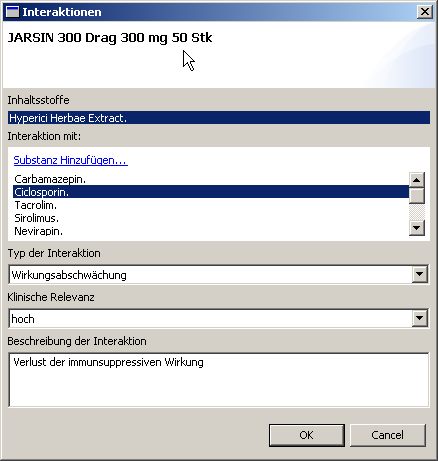
\includegraphics{interakt1}
    \caption{Interaktionen erfassen}
    \label {fig:baginterakt}
    \end{centering}
\end{figure}
Klicken Sie auf einen der im obersten Feld angegebenen Inhaltsstoffe. Es erscheinen dann alle zu diesem Inhaltsstoff bekannten Interaktionen im mittleren Feld. Um eine neue Interaktion zu erfassen, klicken Sie auf \textsc{Substanz hinzufügen}. Wenn Sie eine der Substanzen anklicken, können Sie weiter unten die Art der Interaktion spezifizieren. Geben Sie 'Typ der Interaktion' und 'Klinische Relevanz' ein. Im untersten Feld können Sie die Art der Interaktion noch in Worten beschreiben.

\subsection{Fachinformationen}
Auch hier setzen wir auf \glqq{}do it yourself\grqq{}\footnote{Da dieses Plugin kostenlos ist, rechnen wir mit Ihrem Verständnis dafür, dass es keine teuren Lizenzen für Medikamenteninformationen enthält. Im Prinzip wäre es im Interesse der Qualität des Gesundheitswesens (und damit Sache des BAG) Fachinformationen und Interaktionsdaten zu vernünftigen Preisen zur Verfügung zu stellen. Dies findet bisher aber leider nicht statt.}: Bei denjenigen Medikamenten, die Ihnen wichtig sind, können Sie selbst mit Cut\&Paste die Fachdokumentation hier hineinkopieren. Beachten Sie dabei aber bitte allfällige urheberrechtliche Bestimmungen.

\end{document} 